\documentclass[a4paper,12pt]{article}

% Encoding.
\usepackage[T2A]{fontenc}
\usepackage[utf8]{inputenc}
\usepackage[english,russian]{babel}

% Code insertion.
\usepackage[outputdir=temp]{minted}

% Math functions.
\usepackage{amsmath}

% Image insertion.
\usepackage{svg}


\title{Задание 1: проектирование CLI}
\author{
	Жилкин Феодор\\
	\and
	Смирнов Александр
}
\date{\today}

\begin{document}


\maketitle

\begin{figure}[h]
	\centering
	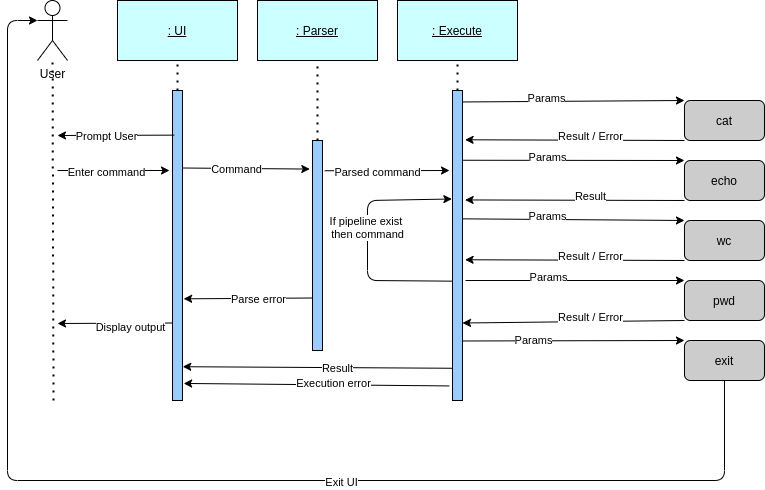
\includegraphics[width=\textwidth]{images/activity_diagram.png}
	\caption{Поведенческая диаграмма}
	\centering
\end{figure}


\newpage

\section*{Схема работы}

\begin{itemize}
	\item UI запрашивает у пользователя входные данные
	\item Пользователь вводит команду
	\item Команда попадает в Parser

	      \begin{itemize}
		      \item Parser разбирает команду
		      \item Проверяет команду на валидность
		            \begin{itemize}
			            \item Если команда валидна, передаем её в Execute
			            \item Если команда не валидна, возвращаем ошибку в UI
		            \end{itemize}
	      \end{itemize}
	\item Если в команде присутствует pipeline, то отправляем на исполнение первую команду
	      \begin{itemize}
		      \item Исполняем команду
		            \begin{itemize}
			            \item Выбираем нужную команду
			            \item Если это exit, то выходим из UI
			            \item Исполняем команду с параметрами
			            \item Если команда выполнилась с ошибкой, возращаем ошибку в Execute, Execute возвращает ошибку в UI
		            \end{itemize}
		      \item Результат команды передаём в Execute в качестве аргумента следующей команде
		      \item Если следующей команды нет, возвращаем результат в UI
	      \end{itemize}
	\item Если в команде отсутствует pipeline, то отправляем команду на исполнение и возвращаем результат в UI
\end{itemize}


\newpage

\section*{Сценарий использования}

Разберём исполнение следующей команды:
\begin{minted}{bash}
cat example.txt | wc
\end{minted}

\begin{itemize}
	\item UI запросил у пользователя входные данные
	\item Пользователь ввёл команду
	\item Команда попала в Parser
	\item Parser разобрал команду, не нашёл ошибок
	\item Parser передал команду в Execute
	\item Execute обнаружил pipeline
	\item Execute подал первую команду до pipeline на исполнение команде cat с параметром example.txt
	\item Команда cat без ошибок выполнилась
	\item Execute получил результат "hello world"
	\item Execute подал вторую команду wc на исполнение команде wc с параметром "hello world"
	\item Команда wc без ошибок выполнилась
	\item Execute получил результат 1 2 11
	\item Execute передал в UI результат
	\item UI отобразил результат
\end{itemize}


\end{document}
